\section{Theoretical Background}
\label{sec:theory}

\subsection{Convolutional Neural Networks}
\label{subsec:cnn}

Convolutional neural networks (CNNs) have excelled at extracting patterns and features from spatial data such as satellite imagery, radar data, and climate model outputs. This capability has enabled researchers to better understand and predict complex atmospheric and oceanic phenomena. For instance, CNNs have been employed to detect and localize extreme weather events from satellite data, enhancing early warning systems and disaster response efforts. Furthermore, CNNs have improved the ability to identify forced climate patterns and disentangle natural variability from human-induced climate change signals, advancing our understanding of climate dynamics and informing mitigation strategies.


CNNs are a type of deep learning architecture inspired by the visual cortex of animals. They are designed to efficiently capture spatial and temporal dependencies in data through the use of learnable filters and hierarchical feature representations. Through the use of convolutional layers instead of fully connected layers, the architecture is able to preserve the spatial structure of the input data, making it particularly well-suited for image and video data. This approach not only simplifies pattern detection but also implies a reduction in the number of parameters, which minimizes the necessary computational resources.

Application of CNNs in climate science has yielded several notable contributions, including the reconstruction of the El Nino event of 1877 by Kadow et al. despite extremely limited data availability. \cite{kadow2020}

In the context of this work an architecture introduced by (\cite{ronneberger2015}) is used, which consists of an encoder and a decoder part as seen in \autoref{fig:u_net}. Due to it's shape it is called U-Net. The encoder part consists of convolutional layers and pooling layers, while the decoder part consists of upscaling layers and in this case, skip connections as proposed by \cite{liu2018inpaining}.

\subsubsection*{Convolutional Layer}
\begin{figure}
    \centering
    \animategraphics[loop,autoplay,width=400pt]{1}{resources/images/convolution_gif/convolution_kernel-}{0}{15}
    \caption{How a convolution operation works. \cite{datahacker}}
    \label{fig:convolution_operation}
\end{figure}

The convolutional layer is the driver for feature mapping in a CNN. It applies a convolution operation shown in \autoref{fig:convolution_operation} to the input data. The operation is done element by element while sliding a filter (also called kernel) over the input data such that situations, where the filter overflows the input data ranges, are avoided or taken care of. On each step, the Frobenius Product between the kernel and the submatrix given by the current position and the kernel dimension is calculated and noted in the output matrix. The parameters in the kernel matrix are chosen in such a way that the Frobenius Product is maximized when the kernel is over a feature that the kernel is supposed to detect. In \autoref{fig:convolution_operation} the kernel for example is a vertical edge detector, meaning it will output a high amount (positive or negative) when the horizontal gradient in the input data submatrix has a high absolute value. This result is rather trivial, as a positive horizontal gradient as seen in the upper-left 3x3 submatrix of the example leads to a right column that when negatively weighted overweights the positive-weighted left column and thus the output for the upper-left 3x3 submatrix is negative. Conversely, a Fresenius product of the upper-right 3x3 submatrix with the kernel returns a positive value, hinting at a negative horizontal gradient in the input data. The result of such a convolution can be observed in \autoref{fig:edge_detection}.

In the context of weather data, the convolutional layer can be used to detect any weather patterns not just edges and the kernel itself can be learned by the network.

\begin{figure}
    \centering
    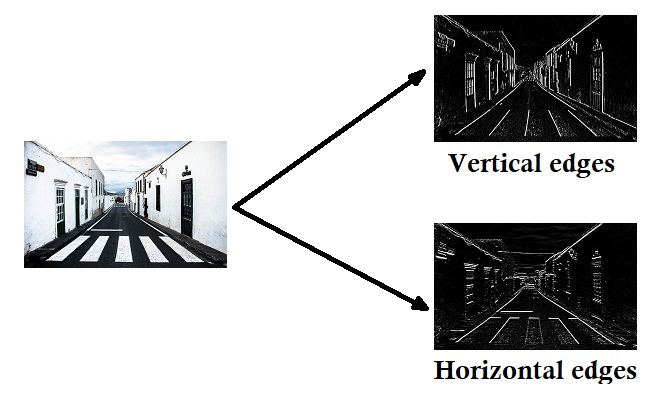
\includegraphics[width=250px]{resources/images/edge_detection.jpeg}
    \caption{Example of edge detection with a convolutional kernel. \cite{datahacker}}
    \label{fig:edge_detection}
\end{figure}

\subsubsection*{Activation Function}

To map the output of the convolutional layer to a meaningful space, and to avoid negative values, an activation function is applied. This introduces non-linearity into the network. The simplest activation function is the ReLU function, which returns the input if it is positive and zero otherwise. It is defined as $f(x) = max(0, x)$. The ReLu function is the activation function used in this work after each convolutional operation.

\subsubsection*{Pooling Layer}

The exact position of a low-level feature in the input data is not so important when it comes to detecting high-level features,
it is more important to recognize if a feature is present at all in certain spatial areas of the input data or not.
Thus scaling down the resolution of the matrix by combining every 2x2 submatrix into one value can be beneficial.
It is most commonly aggregated by taking the maximum value of the submatrix because it works for the mentioned purpose to detect if a feature is present in the area of the submatrix or not. While the convolution layer depending on how the convolution is processed near the borders of the input data reduces the dimensionality of the input data just slightly or not at all, the pooling reduces the dimensionality drastically. So after a 2x2 pooling operation, the output matrix is only a quarter of the size of the input matrix.

\begin{figure}
    \begin{subfigure}{1\textwidth}
        \centering
        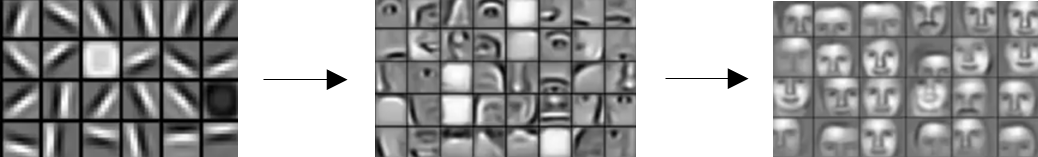
\includegraphics[width=0.9\textwidth]{resources/images/abstraction.png}
        \caption{Low-level features are combined into high-level features.}
        \label{fig:abstraction}
    \end{subfigure}
    \vspace{0.5cm}
    \begin{subfigure}{0.65\textwidth}
        \centering
        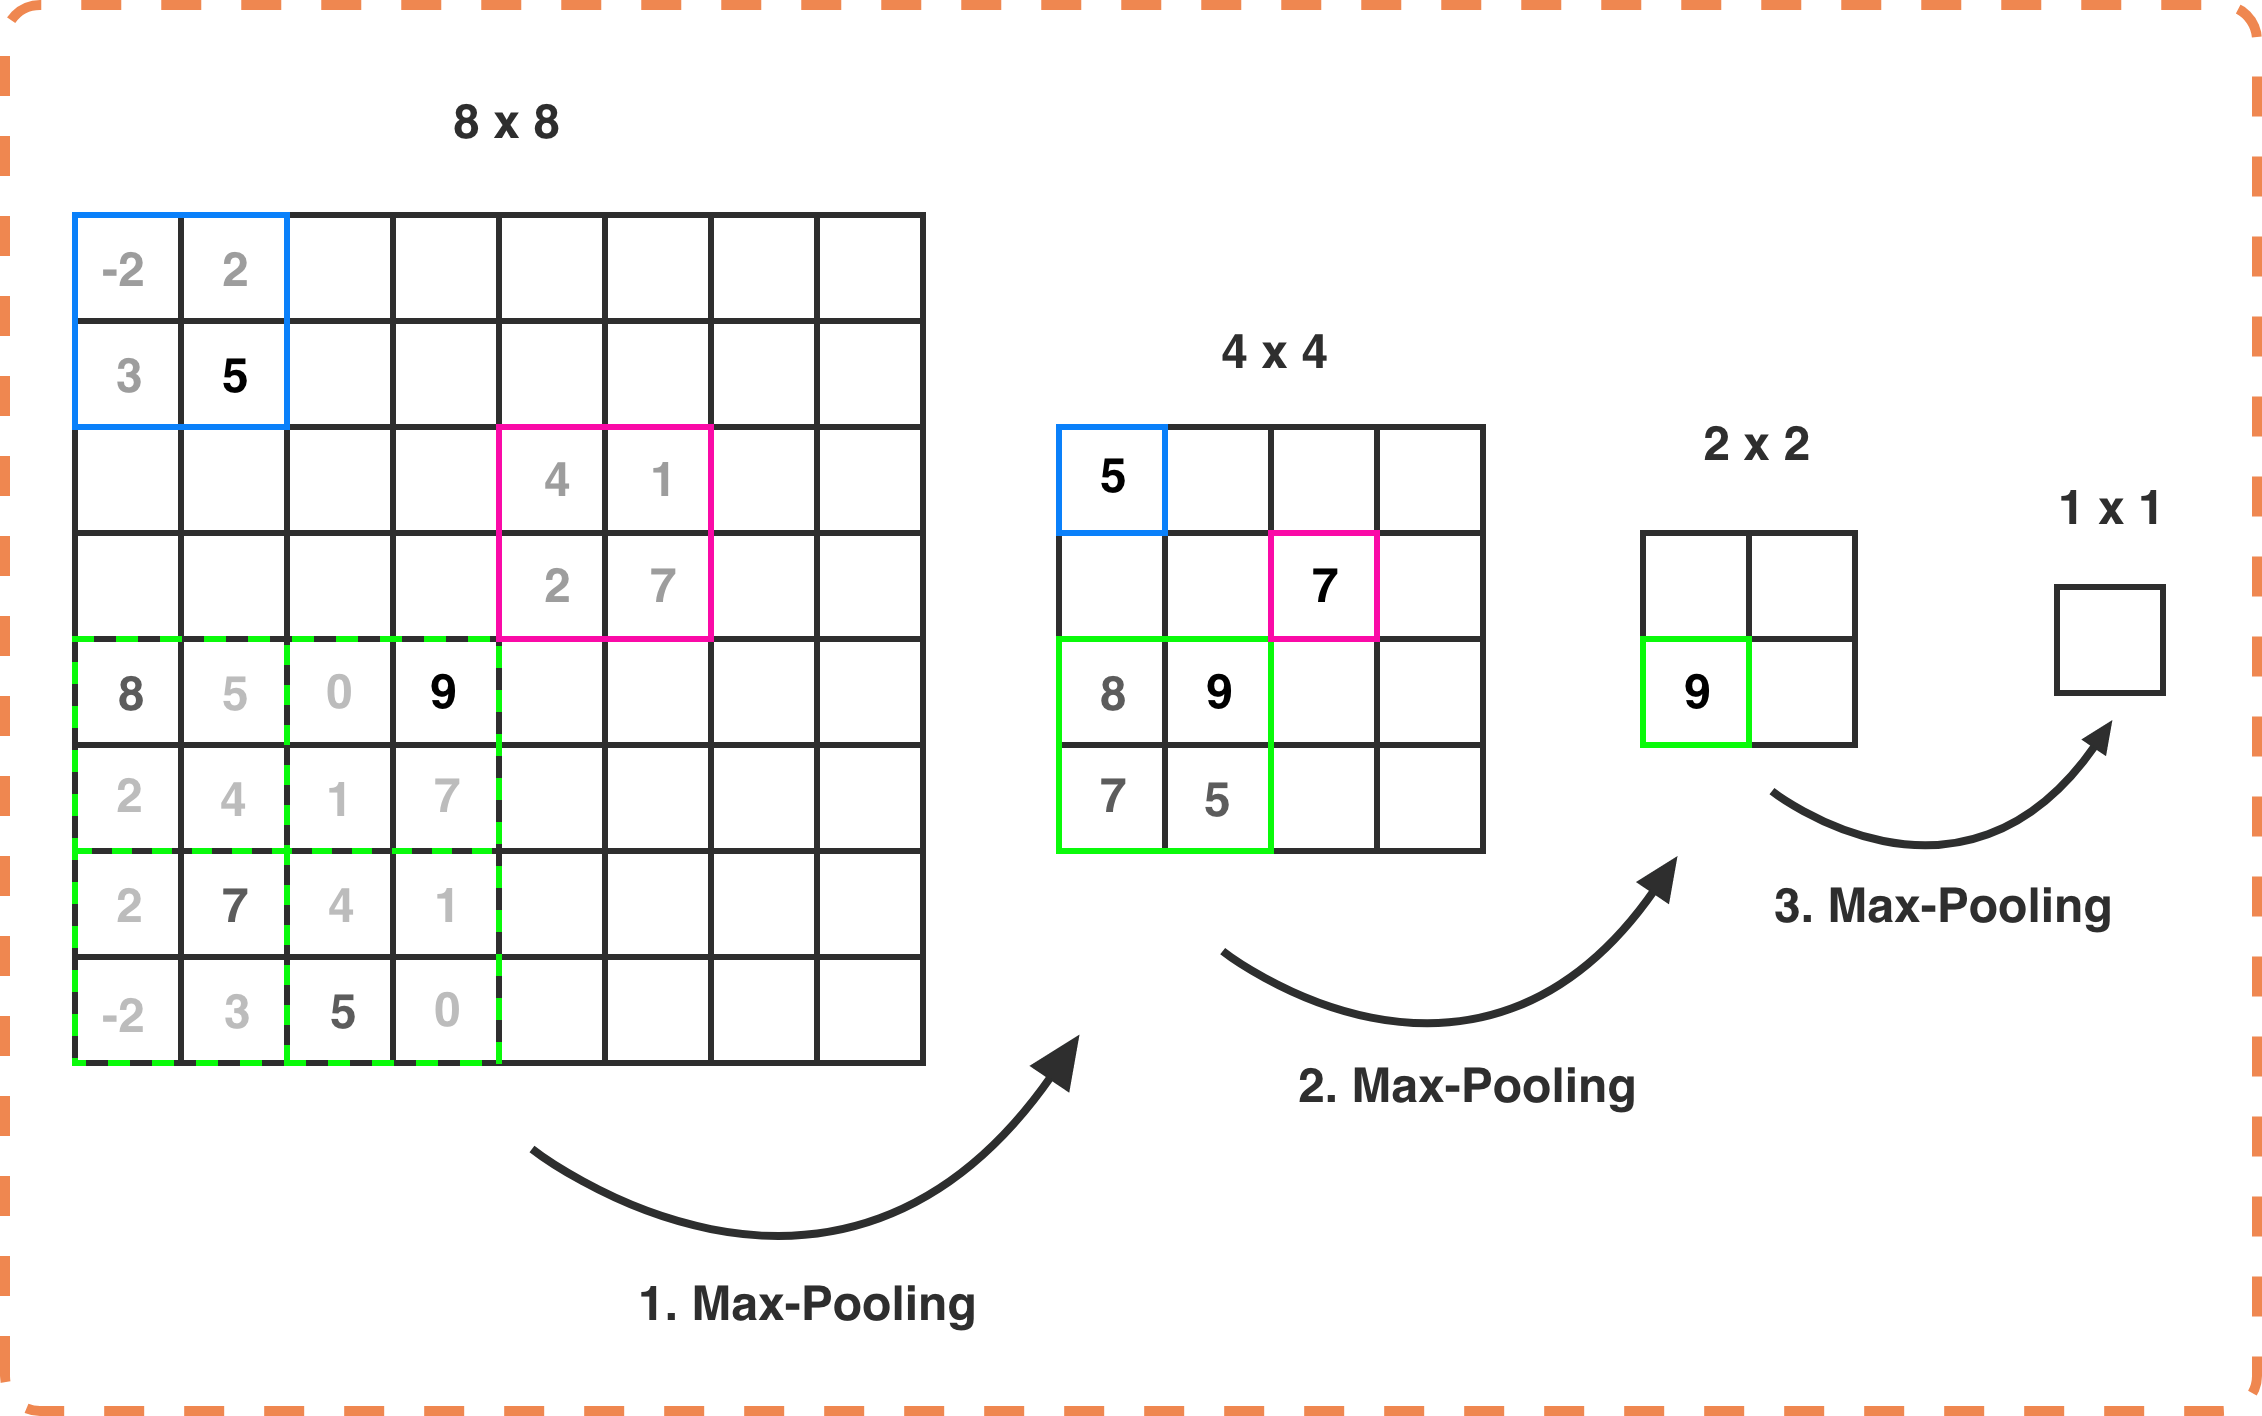
\includegraphics[width=\textwidth]{resources/images/max_pooling.png}
        \caption{Illustration of 3 max pooling operations}
        \label{fig:max_pooling}
    \end{subfigure}
    \begin{subfigure}{0.30\textwidth}
        \centering
        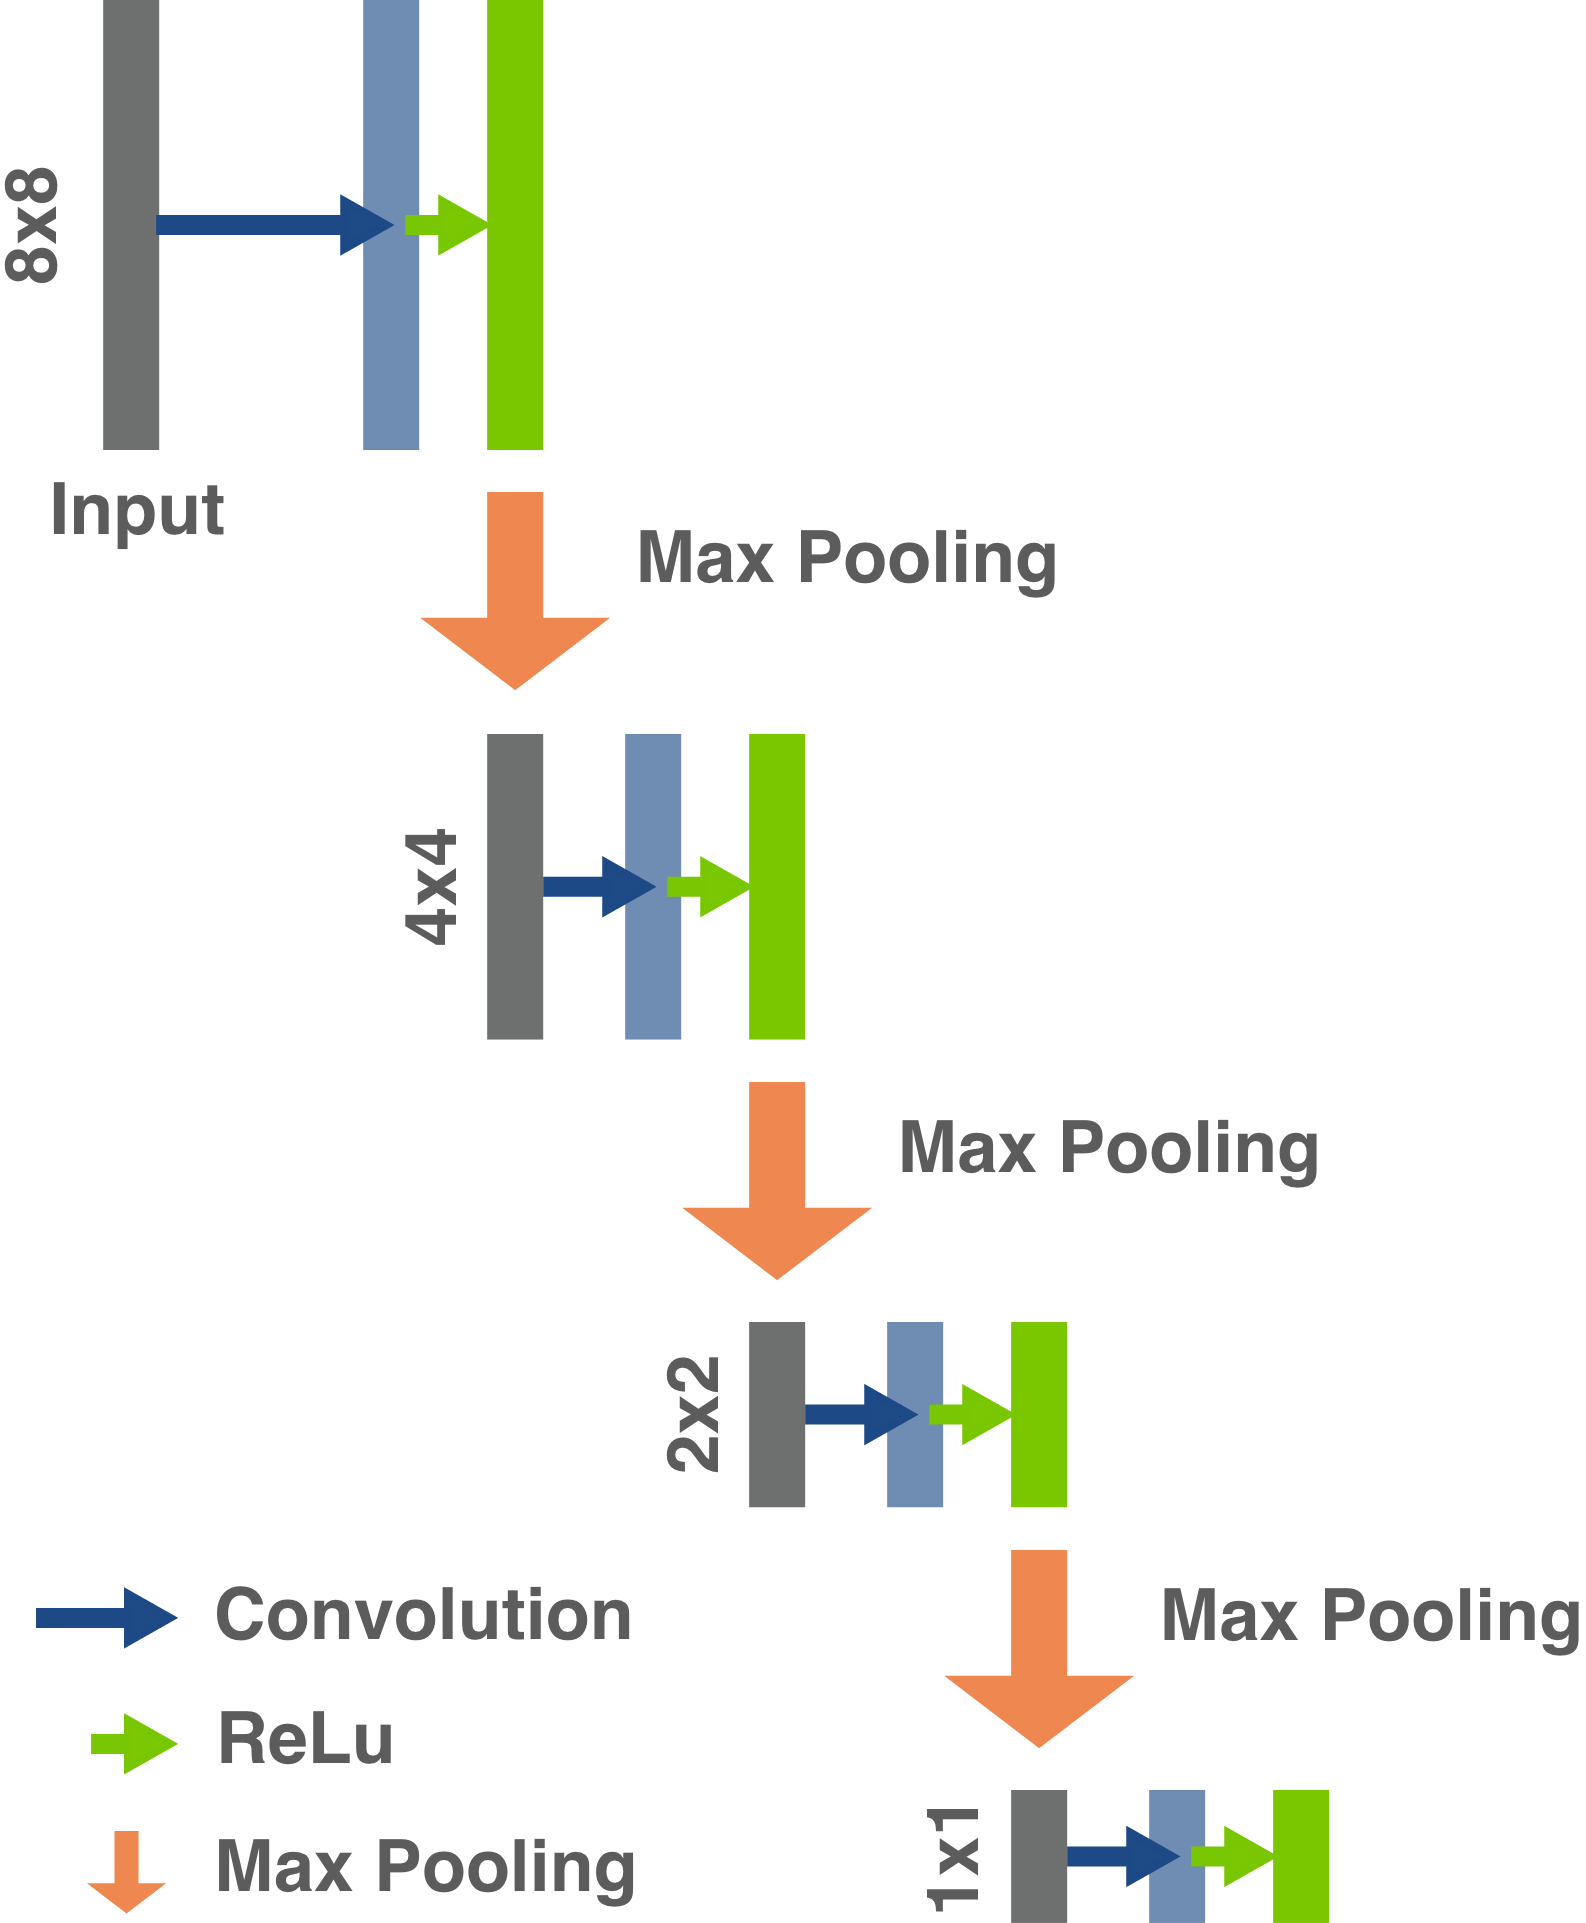
\includegraphics[width=\textwidth]{resources/images/encoder_architecture.png}
        \caption{Alternation of convolutional and pooling}
        \label{fig:encoder_architecture}
    \end{subfigure}
    \caption{Abstraction in the encoding part of a CNN.}
\end{figure}


For the 8x8 grid cells of the ERA5 data, that is used as input in the laid out approach (see \autoref{subsec:data_preprocessing}), the architecture of the CNN could include a maximum of 3 pooling layers, reducing the input data to a 1x1 matrix as seen in \autoref{fig:max_pooling}. \autoref{fig:max_pooling} just illustrates the downsampling of the data, in the actual architecture pooling layers always follow convolutional layers and are never applied directly after each other as seen in \autoref{fig:encoder_architecture}. 


\begin{figure}
    \centering
    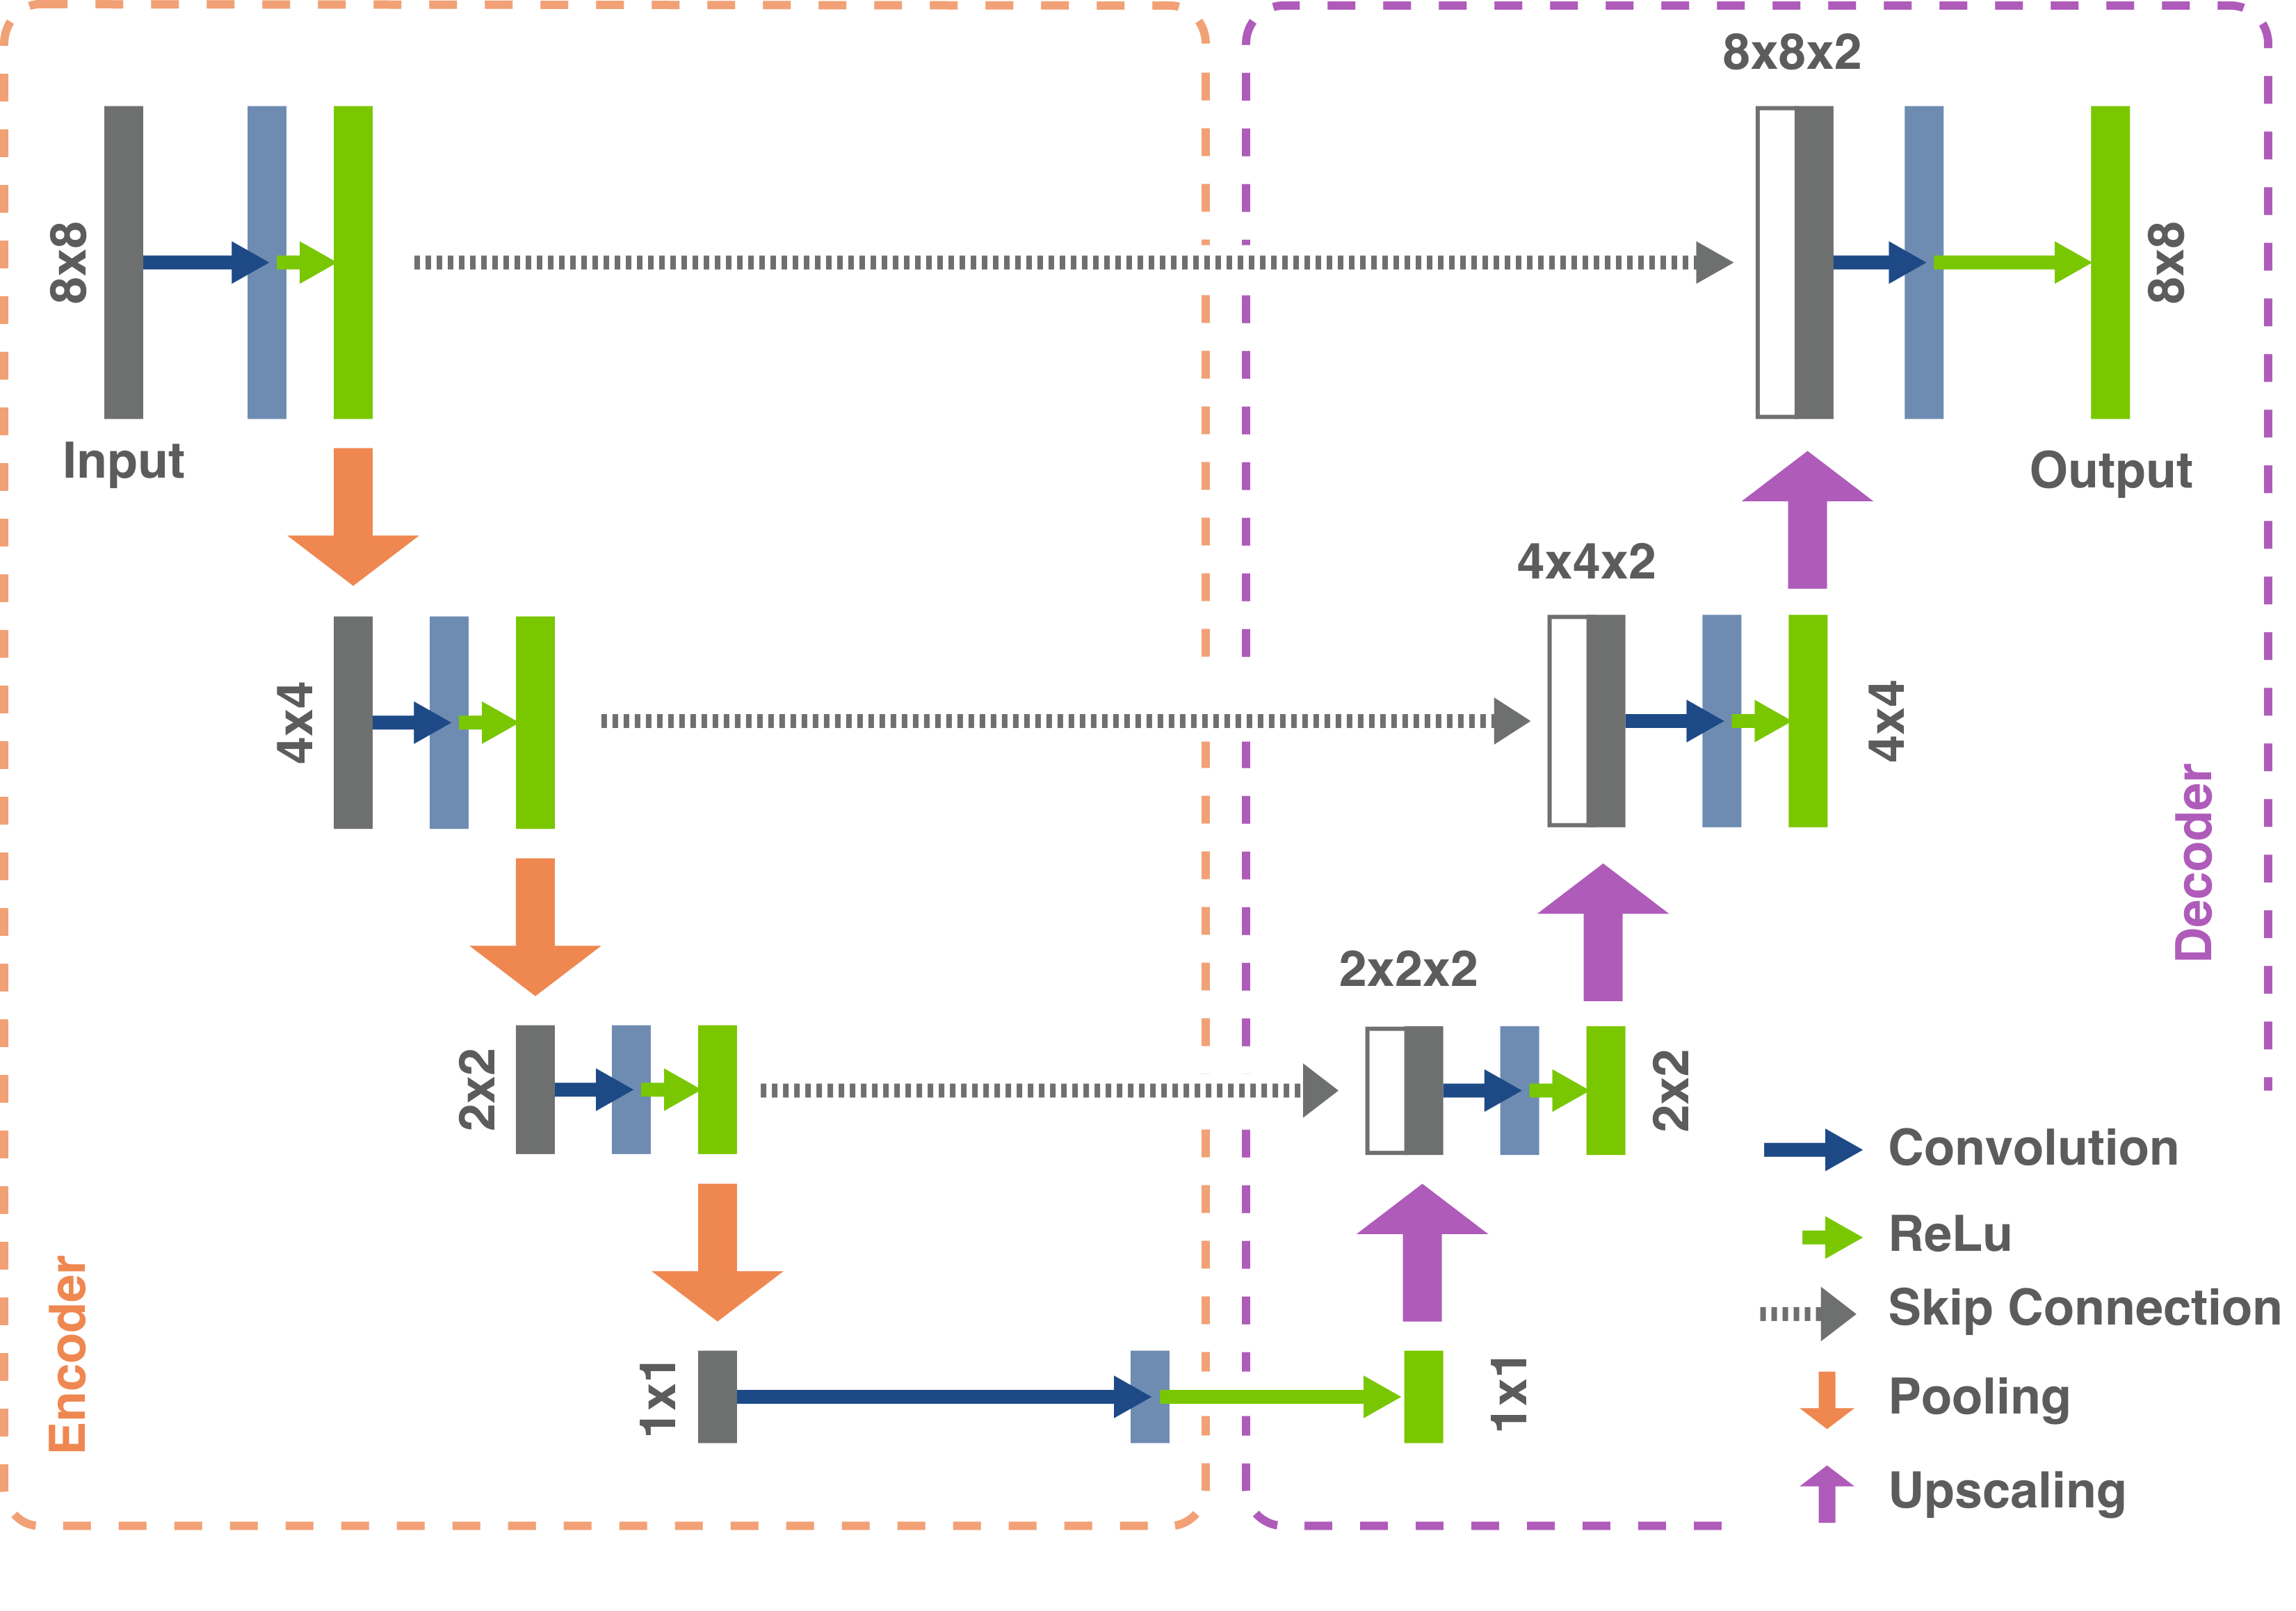
\includegraphics[width=0.9\textwidth]{resources/images/u_net.png}
    \caption{Encoder Decoder Architecture in the U-Net.}
    \label{fig:u_net}
\end{figure}

\subsubsection*{Upscaling Layer}

In the decoding part of the U-Net, the shape of the data is restored by upscaling the encoded layers with the detected feature again. This is simply done through Gaussian interpolation.

?? Question: What else can I explain here?

A very important part of the decoder is the usage of skip connections (\cite{liu2018inpaining}). 

\subsubsection*{Skip Connections}

??? Question is this even helpful when not infilling but using "target" data as input?

For the skip connections, the outputs on each layer of the encoding part are copied over and directly factored into the decoding part. This helps the network to remember the context of the input data, helping to preserve the context of the input data, which is especially important in spatial infilling tasks, where the reconstruction needs to match the available data around the missing data. To combine the data from the skip connections with the data from the upscaling layers, a specialized convolution is used... 

?? Question: Is this correct? Or Convolution->ReLU + Pooling? How is the dimensionality halved again?

The now-explained steps used in the architecture combined will return for any input data a prediction of the same shape as the input data, where the values are the predicted values for the missing data. What the values exactly will be is completely dependent on the parameters used in the convolution kernels.


?? Question: What else weights are there? The architecture does not have fully connected layers, does it? So no weights there. What about the pooling and upscaling layers? Are there weights in the activation function?

With the correct weights found the prediciton should be ideally the same as the target data. This is what the training process is for which is supervised based on the available measurements, the ground truth (see \autoref{fig:supervised_learning}). 

\subsubsection*{Backpropagation and Loss Function}

??? I am using Loss Function 3, what should I explain here in the context of a bachelor thesis about it?

To minimize any differences between ground through and prediction, the differences first need to be quantified in a loss function. Then the partial gradient of the loss function concerning each weight in the network is calculated. This is done through backpropagation, recursively applying the chain rule of calculus. The weights are then updated in the opposite direction of the gradient, such that the loss function is minimized. The learning rate determines how big the adjustments are made and is a crucial hyperparameter in the training process. 


\begin{figure}
    \centering
    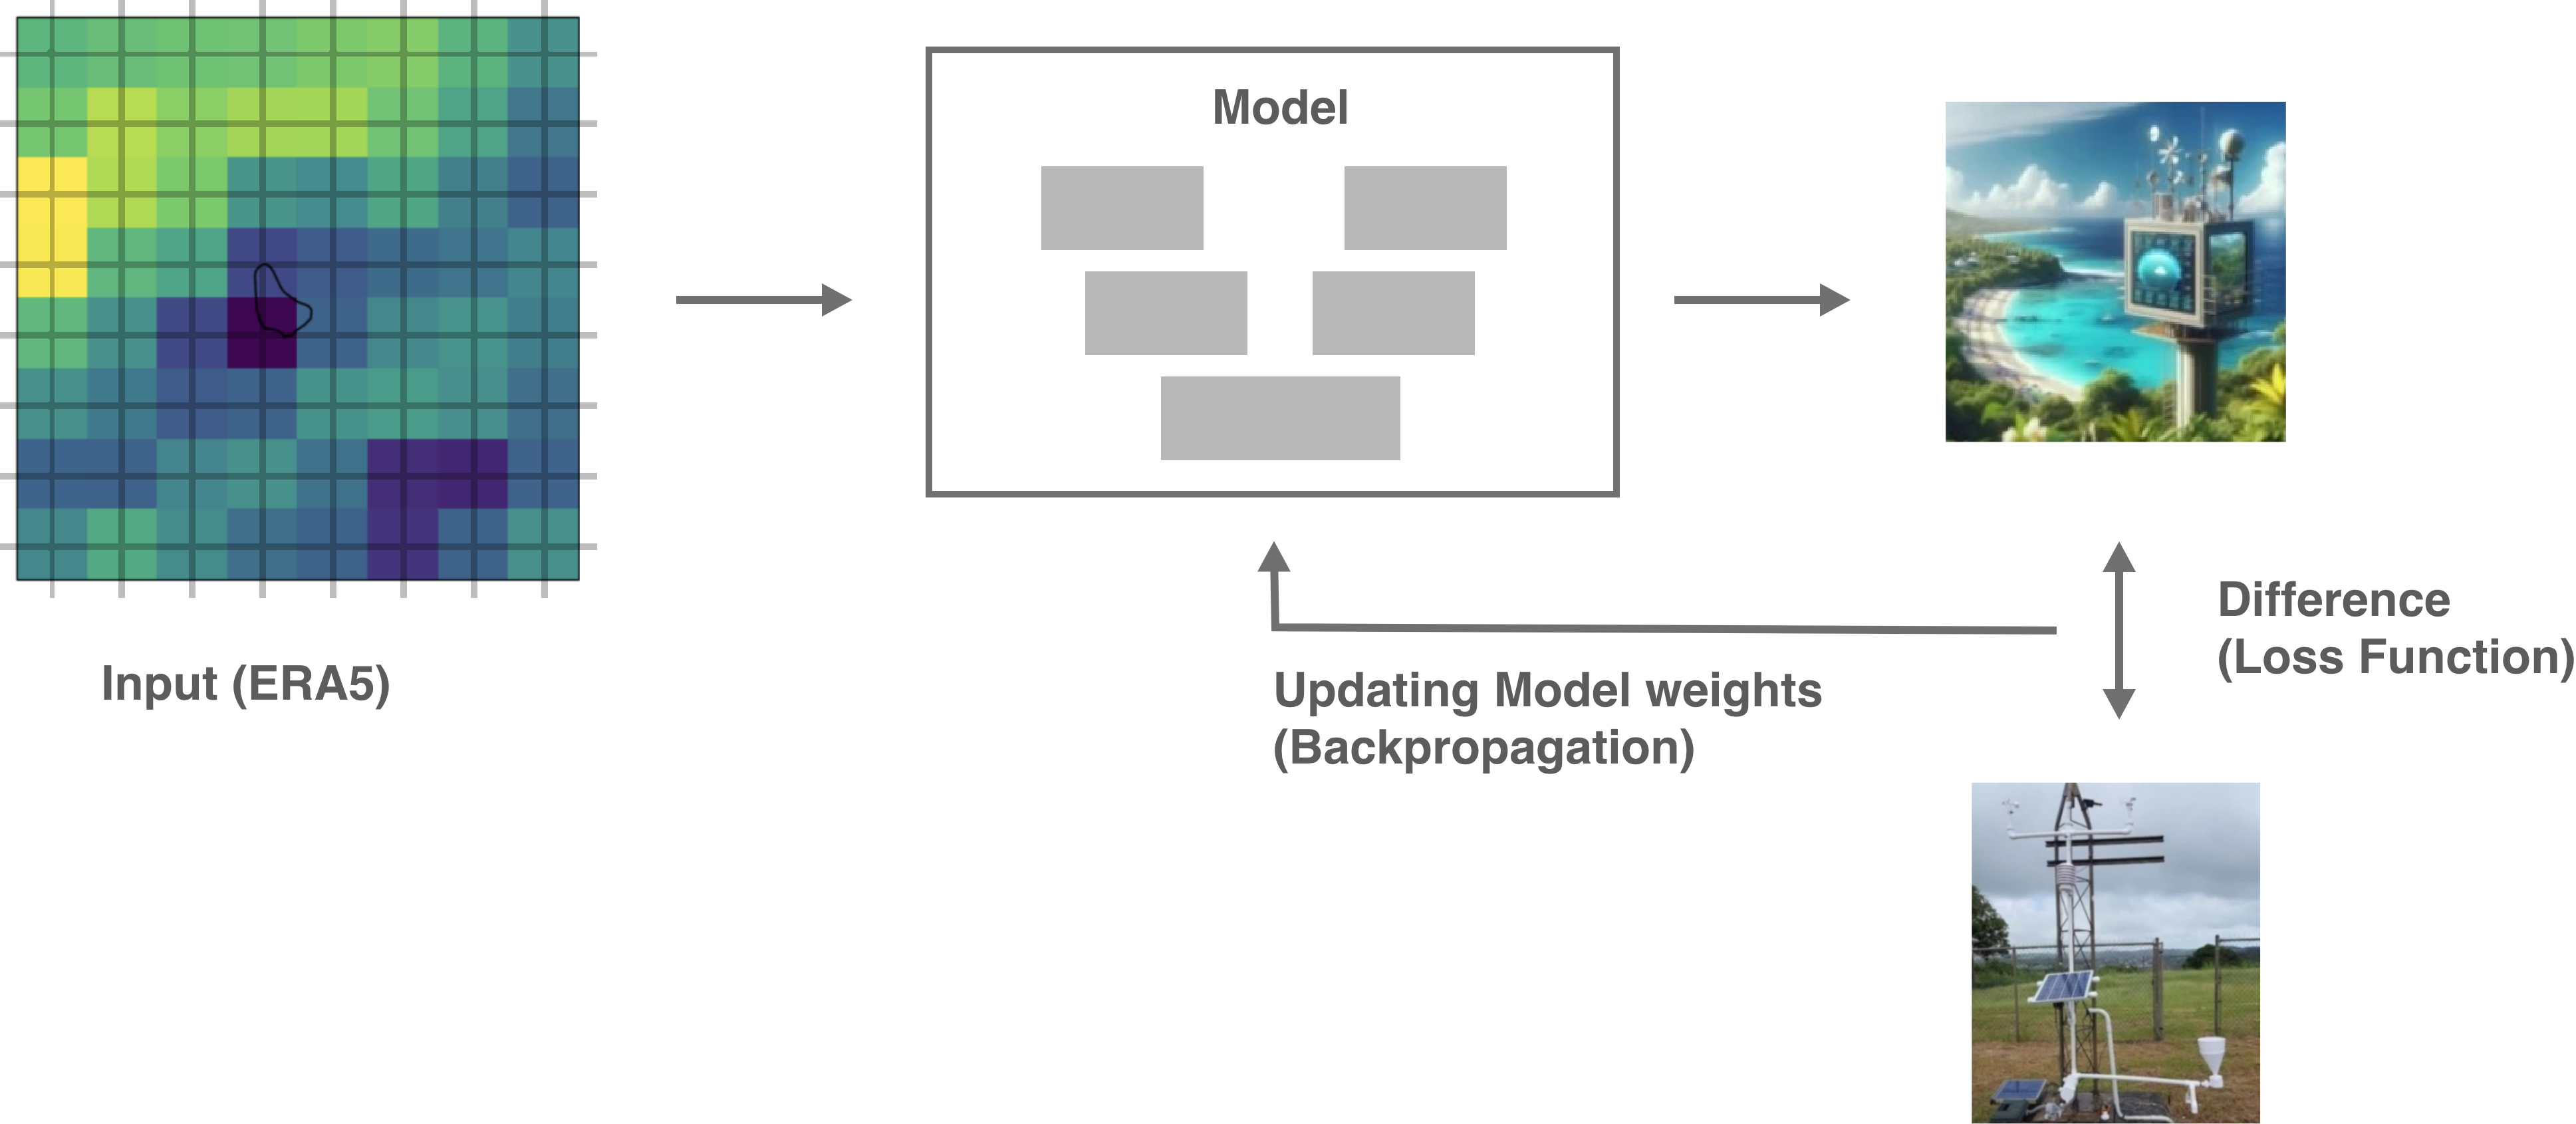
\includegraphics[width=0.9\textwidth]{resources/images/supervised_learning.png}
    \caption{Schema of supervised learning.}
    \label{fig:supervised_learning}
\end{figure}


\subsection{Reanalysis - ERA5}

Atmospheric reanalysis is an effort to combine measurements with numerical models to estimate the state of the atmosphere at any given time, opposing missing measurements. The method is based on a complex numerical model, simulating the physical rules of the atmosphere. As with any numerical model, degrees of freedom, allow for adjustments of parameters, which are chosen in such a way that the model output matches the actual measurements wherever they are available in space and time. 

The ERA5 reanalysis is a product of the European Centre for Medium-Range Weather Forecasts (ECMWF) and is the fifth generation of the ERA reanalysis series. It is the most complete and accurate data assimilation project available \cite{Hersbach2020ERA5quality}. Which makes it the best choice as input data in this approach. As it is the best available data in remote locations such as in East Africa \cite{Gleixner2020ERA5africa}, where the 3D printed weather stations are specifically supposed to make an impact it can be used as a type of benchmark to compare the results of the infilling approach to.

As mentioned above the data is available in grid cells of 0.25° x 0.25°, which is approximately 28 km x 28 km at the equator. The data assimilation takes place in 4 dimensions, as not only the latitude and longitude over time are taken into account but also multiple pressure levels in the atmosphere. This gives the techniques used for ERA5 the name 4D-Var \cite{era5}
The available variables in the ERA5 reanalysis are numerous, but for this work, only the 2m temperature is used as input to the neural network. Which is the temperature weather stations aim to measure. However, for similar approaches or extended approaches, other variables such as different wind-(component) speeds, precipitation, or humidity and solar radiation could be used as well.